\subsection{单通道随机性模型}
\subsubsection{理论分析}
考虑非高峰期的情况下,使用一个参数为$\lambda_{l}$的泊松过程来表示顾客源,
使用负指数分布的随机服务时长,即$M/G/1/\infty/\infty/FCFS$模型。
其中使用的是G而不是M是因为总的服务时长$t_{all}=2t_{c}+t_{r}$,是一个
符合负指数分布的变量加上一个常量,并不是严格的负指数分布,所以用一般分布G表示。
\par 对本模型的求解,主要按照按模型1的求解方法,先建立对应稳态之间的差分方程:
\begin{equation}
    \begin{aligned}
        \lambda P_{n-1}(t)+\frac{\mu}{2t_c\mu+1} P_{n+1}(t)-(\lambda+\frac{\mu}{2t_c\mu+1} )P_n(t)& =0,n\geq 1 \\
        -\lambda P_{0}+\frac{\mu}{2t_c\mu+1} P_{1}&=0
    \end{aligned}
\end{equation}
求解这个差分方程可以得到对应状态的概率
\begin{equation}
    \begin{aligned}
        P_0 &=1-\rho \\
        P_n &=(1-\rho)\rho^n,n\geq1
    \end{aligned}
\end{equation}
其中的$\rho=2\lambda t_c+\frac{\lambda}{\mu}$,它的物理意义为服务强度。
随后,通过与模型1类似的方法可以得到对应状态转移关系。
图\ref{fig:transform2}中展示了不同状态转移关系。
\begin{figure}[ht]
    \centering
    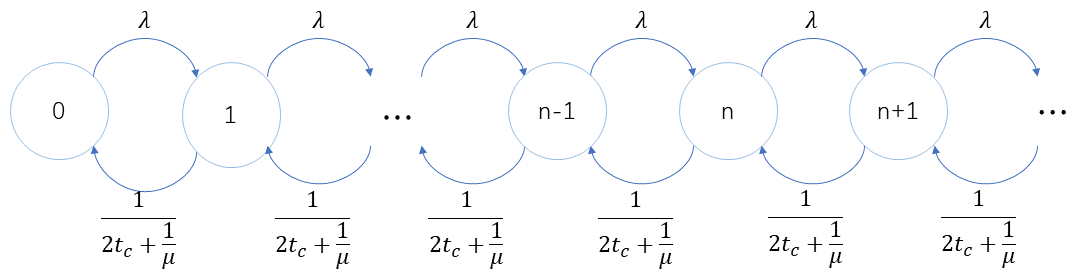
\includegraphics[width=.6\textwidth]{images/transform2.PNG}
    \caption{随机模型单通道状态转移图}
    \label{fig:transform2}
\end{figure}
\par 对于默认关门的情况,服务时间是$t_1=2t_c+\frac{1}{\mu}$,
所以服务强度$\rho_1=2t_c\lambda_l+\frac{\lambda_l}{\mu}$,
得到理论上的平均队长$L_s=\frac{\rho_1}{1-\rho_1}$。
\par 同理,对于默认开门的情况,服务时间是$t_2=t_r+t_{penal}$,
$t_{penal}$表示刷卡失败的惩罚时间,惩罚时间的建模与上一个模型一致。

其中$p_o$为开门成功率。$T_{penal}$为惩罚的具体时间大小。
这里的$t_r$与$t_{penal}$是相互独立的,因为后者是否存在仅仅取决于是否刷卡失败,
而这对随机服务时间,即刷卡时间与经过时间,没有任何影响。从而得到总服务时间的期望与方差如下:
\begin{equation}
    \begin{aligned}
        E(t_2) &=\frac{1}{\mu}+(1-p_o)T_{penal} \\
        Var(t_2)&=\frac{1}{\mu^2}+p_o(1-p_o)T_{penal}^2
    \end{aligned}
\end{equation}

所以服务强度$\rho_2=\lambda_l (1-p_o)T_{penal}+\frac{\lambda_l}{\mu}$,
直接运用Pollaczek-Khintchine公式得到理论上的平均队长
$L_s=\rho_2+\frac{\rho_2^2+\lambda^2/\mu^2+\lambda^2 p_o(1-p_o)T_{penal}^2}{2(1-\rho_2)}$
\par 最后将两者比较,得到两种服务方式的平均队长的比值
\begin{equation}
    \begin{aligned}
        \frac{L_{s1}}{L_{s2}}&=\frac{\frac{\rho_1}{1-\rho_1}}{\rho_2+\frac{\rho_2^2+\lambda_l^2/\mu^2+\lambda_l^2 p_o(1-p_o)T_{penal}^2}{2(1-\rho_2)}} \\
        &=\frac{2\rho_1(1-\rho_2)}{(1-\rho_1)[2\rho_2-\rho_2^2+\lambda_l^2/\mu^2+\lambda_l^2 p_o(1-p_o)T_{penal}^2]}
    \end{aligned}
\end{equation}
其中$\rho_1=2t_c\lambda_l+\frac{\lambda_l}{\mu}$,
$\rho_2=\lambda_l (1-p_o)T_{penal}+\frac{\lambda_l}{\mu}$
\par 对结果进行简单的讨论:
\begin{itemize}
    \item 对于服务强度,$\rho_1-\rho_2=\lambda_l(2t_c-(1-p_o)T_{penal})$,
    由于$p_o$是一个很大的值,一般在0.9以上,所以默认关门的服务强度
    比默认关门要大得多,即在人流相同的条件下,默认开门的通行压力要更小。
    \item 对于这个公式,给出我们接下来数值时使用的参数,代入公式进行计算,
    具体取值如下:$t_c=0.5$,$\mu=1$,$p_o=0.9$,$T_{penal}=1$,$\lambda_l=0.2$,
    则$\rho_1=0.4,\rho_2=0.22$,从而$L_{s1}=\frac{2}{3},L_{s2}=0.278,\frac{L_{s1}}{L_{s2}}=2.4>1$。
    所以一般默认开门的平均队长是默认关门平均队长的0.42倍。
    也可以根据Little法则算出对应的等待时间比值,与平均队长的比值是一致的。
\end{itemize}
\subsubsection{模型建立与求解}
在确定性模型中,刷卡时间和通行时间(之后统称为服务时间)认为是常数,
在实际情况中,服务时间往往会因为客户对象的不同而发生变化。
选择利用负指数分布刻画这种服务时间的不确定性,从而更好地刻画队伍的运动情况。
\par 由于负指数分布可能给出过大的服务时间值,在数值模拟时将负指数分布产生的
随机数限制在区间$[t^*, 6 t^*]$内,其中$t^*$为模拟的时间步长。
数值模拟过程中,参数取值为:
\begin{itemize}
    \item 道路长度为40
    \item 生成对象的过程服从$\lambda_l = 0.2$的泊松分布
    \item 对于生成的对象,是行人的概率为0.8,是自行车的概率为0.2
    \item 负指数分布的参数$\mu = 2t^*$
    \item 刷卡成功率为0.9
    \item 模拟次数为10000,每隔4次记录平均队长
\end{itemize}
同时在人的生成部分,采用一个缓冲区存储没有能够立刻进入队伍的人。
模拟得到平均队长的变化(30步移动平均)记录在图\ref{fig:average-length-with-exp}中。
\begin{figure}[ht]
    \centering
    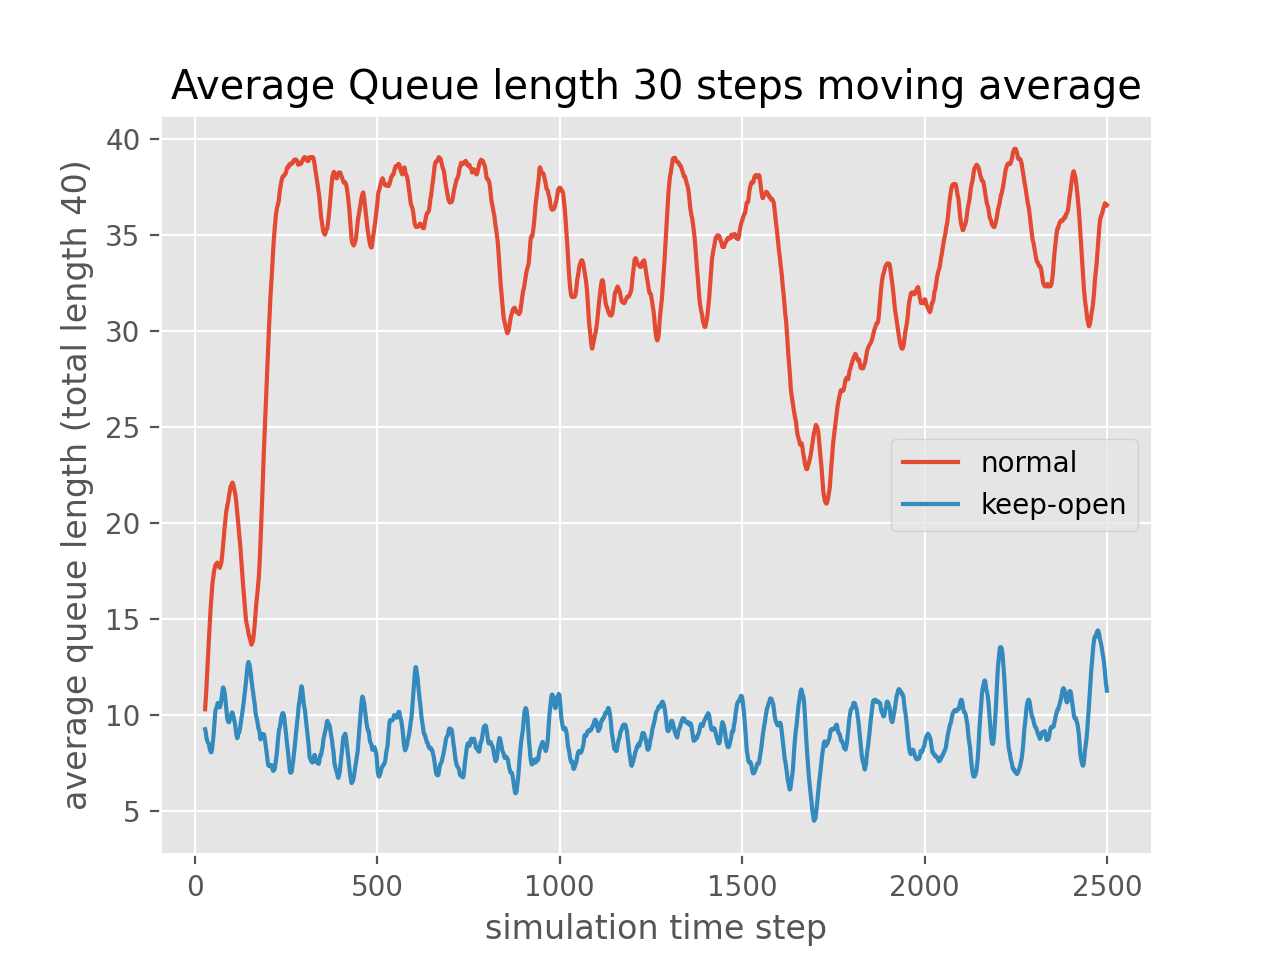
\includegraphics[width=.6\textwidth]{images/avg_queue_length_with_exp.png}
    \caption{服务时间满足负指数分布的平均队长,其中红线为校门的正常开关状态,蓝线
    为校门保持开放}
    \label{fig:average-length-with-exp}
\end{figure}
图\ref{fig:average-length-with-exp}相较图\ref{fig:queue-length-time}
少了很多人数直线下降的情况,说明缓冲区的选取更加符合实际。
观察到校门正常开放的队伍平均长度明显大于校门保持开放时的平均长度。
在遇到服务时间较长的情况时,由于不能换道,队伍很容易出现充满的情况,造成平均队长保持在
一个较大的值,此时门常开对于通行效率的优势体现的更为明显。
\par 刷卡成功率对于两种通行方式的效率有很大的影响,将成功率下调为0.4后,得到的
平均队长的比值(常开/正常)关于模拟次数的曲线展示在图\ref{fig:low-success-rate}中。
\begin{figure}[ht]
    \centering
    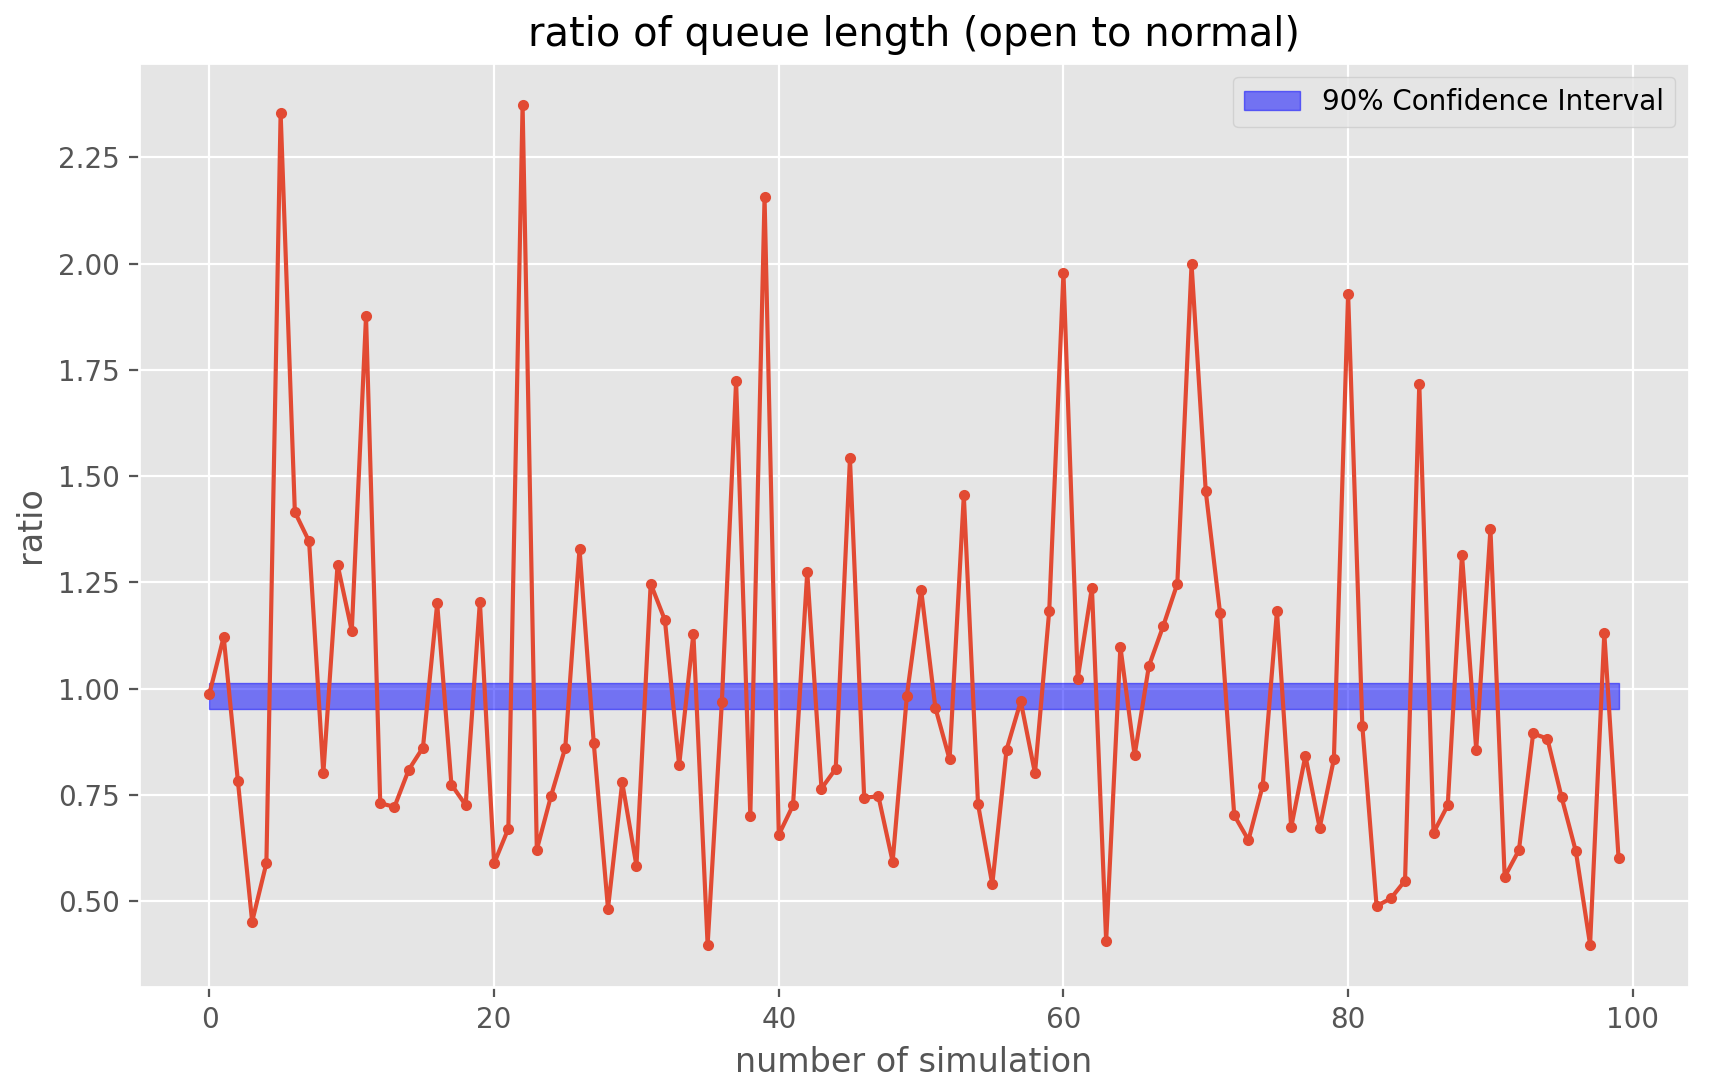
\includegraphics[width=.7\textwidth]{images/ratio_low_success_rate.png}
    \caption{成功率为0.4时的平均队长比值(常开/正常)与比例平均值90\%置信区间}
    \label{fig:low-success-rate}
\end{figure}
从图\ref{fig:low-success-rate}中明显观察到,比例均值的置信区间由之前的0.45上升到接近
1,说明两种方法在刷卡失败率较高时通行效率相差不大。但是如果进一步考虑安全性、便于管理性,
门正常开关在这种情况下好于门保持开放。